\section{Traffic Light Control}

\begin{frame}{TLC as MDP}
RL learns to maximize expected total reward in an MDP (best case)

        \begin{itemize}
            \item \alert{construct state signal}
            \item determine reward function
            \item chose set of actions
            \item simulate environment dynamics
        \end{itemize}


\end{frame}

\begin{frame}{Markovian Road Users}
   \includegraphics[height=\textheight,width=\textwidth,keepaspectratio]{1balls}
\end{frame}
\begin{frame}{Markovian Road Users}
   \includegraphics[height=\textheight,width=\textwidth,keepaspectratio]{2balls}
\end{frame}
\begin{frame}{Markovian Road Users}
   \includegraphics[height=\textheight,width=\textwidth,keepaspectratio]{3balls}
\end{frame}
\begin{frame}{Markovian Road Users}
   \includegraphics[height=\textheight,width=\textwidth,keepaspectratio]{4balls}
\end{frame}
\begin{frame}{Markovian Road Users}
   \includegraphics[height=\textheight,width=\textwidth,keepaspectratio]{5balls}
\end{frame}
\begin{frame}{Markovian Road Users}
   \includegraphics[height=\textheight,width=\textwidth,keepaspectratio]{allballs}
\end{frame}

\begin{frame}{Markovian Road Users}
\begin{table}[]
\centering
\caption{My caption}
\label{intersection state}
\begin{tabular}{@{}lll@{}}
\toprule
frames & information  & order \\ \midrule
1      & position     & 0     \\
2      & velocity     & 1     \\
3      & acceleration & 2     \\
4      & jerk         & 3     \\
5      & jounce       & 4     \\ \bottomrule
\end{tabular}
\end{table}
\end{frame}


\begin{frame}{Markovian Road Users}
          \begin{columns}[c,onlytextwidth]
    \column{0.5\textwidth}
\begin{equation*}
s= \begin{bmatrix}
           1 \\
          0 \\
           5\\
           4
         \end{bmatrix}
\end{equation*}
    \column{0.5\textwidth}
    \begin{figure}
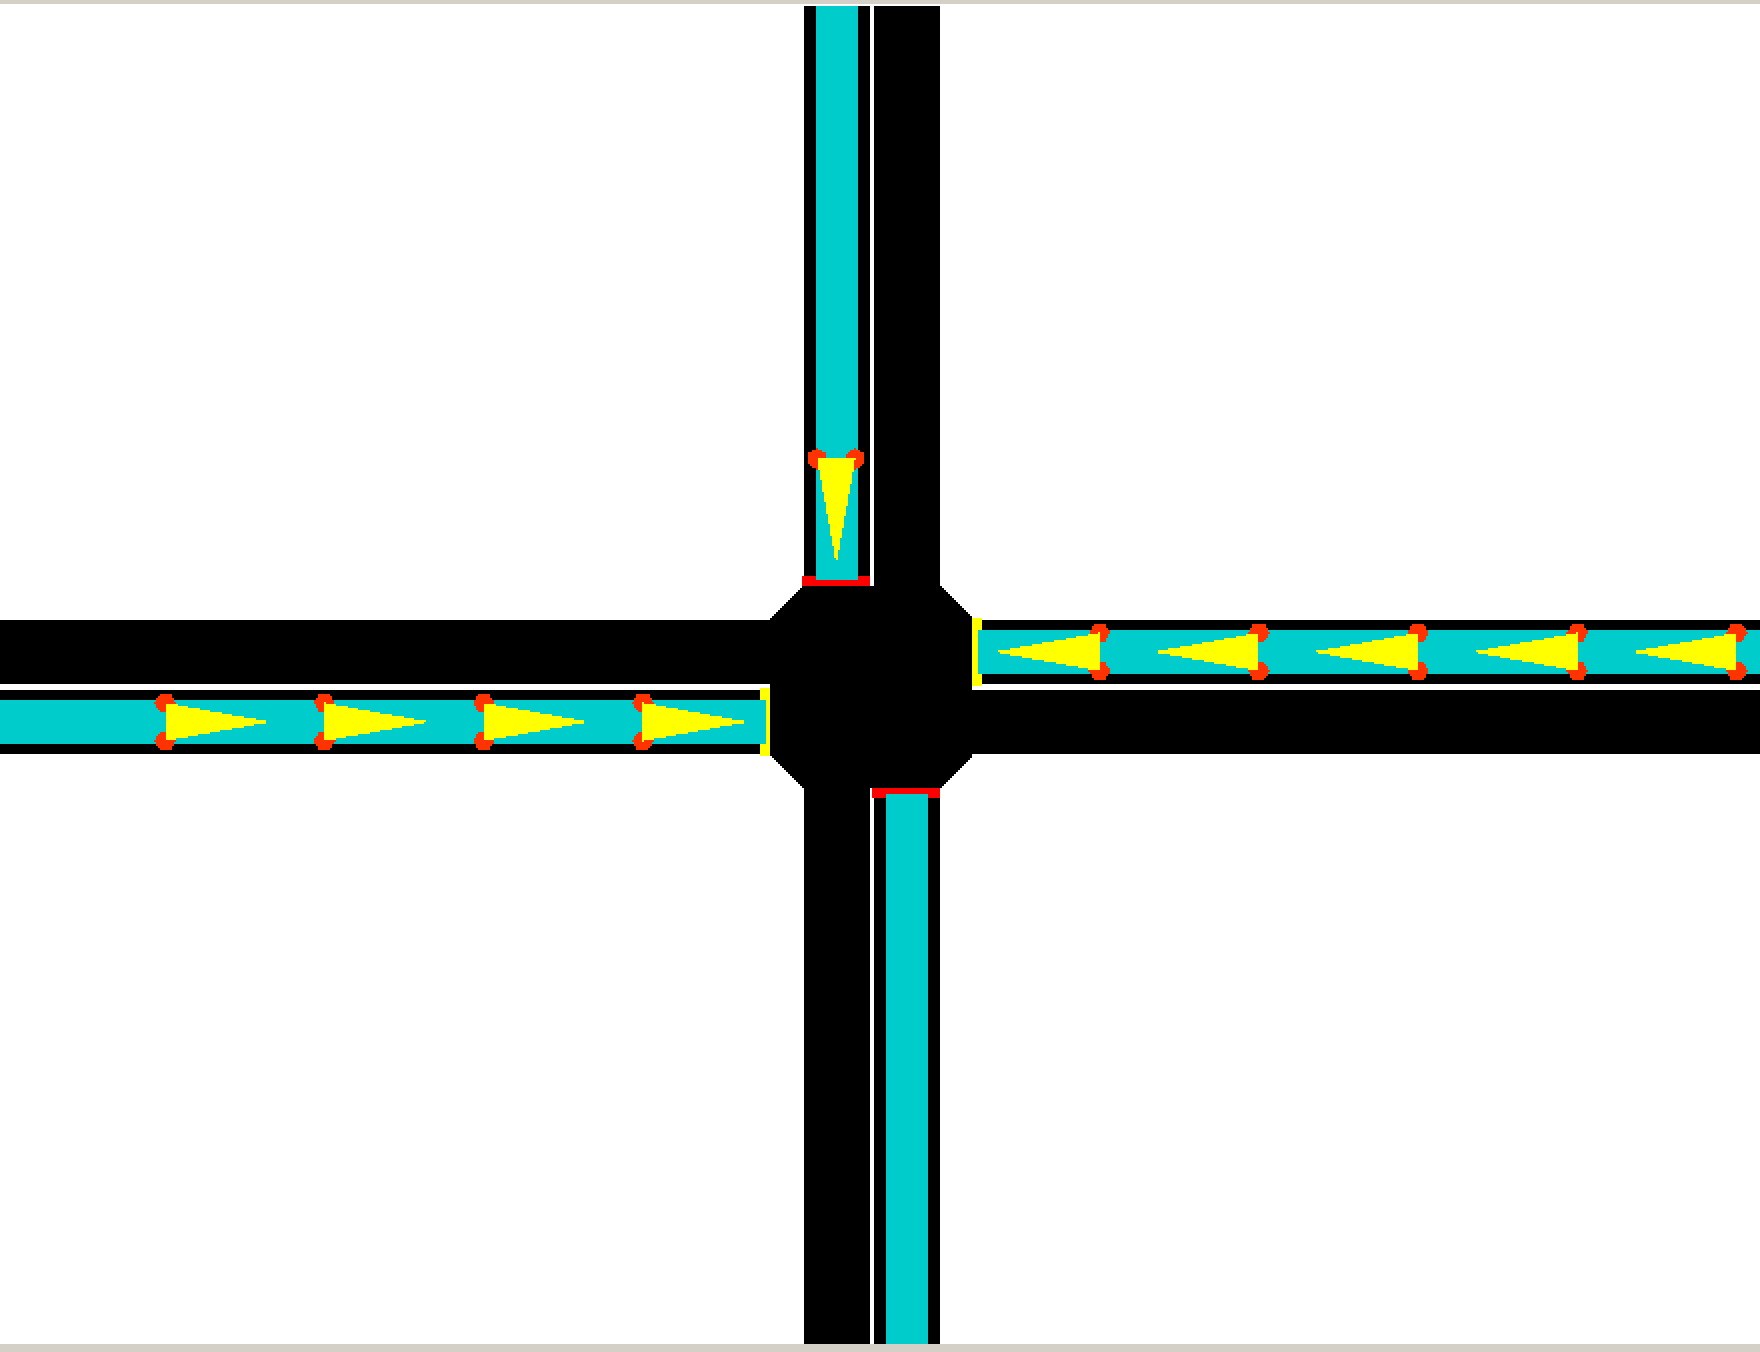
\includegraphics[width=\textwidth]{queue}
\caption{intersection with 4 approaches}
    \end{figure}
        

  \end{columns}
\end{frame}

\begin{frame}
\begin{figure}
\begin{tabularx}{\textwidth}{|X|X|X|X|X|X|X|X|X|X|X|X|}
\hline
1 & 1 & 1 & 0 & 1 & 0 & 0 & 0 & 0 & 0 & 0 & 0 \\ \hline
0.01 & 0.07 & 0 & 0 & 0.68 & 0 & 0 & 0 & 0 & 0 & 0 & 0 \\ \hline
\end{tabularx}

\includegraphics[width=\textwidth]{moving}
\caption{Crop used for demonstrating different state representations}
\end{figure}
\end{frame}
\begin{frame}
\begin{figure}
\begin{tabularx}{\textwidth}{|X|X|X|X|X|X|X|X|X|X|X|X|}
\hline
1 & 1 & 1 & 1 & 1 & 1 & 0 & 0 & 0 & 0 & 0 & 0 \\ \hline
0 & 0.07 & 0.16 & 0.1 & 0.05 & 0 & 0 & 0 & 0 & 0 & 0 & 0 \\ \hline
\end{tabularx}

\includegraphics[width=\textwidth]{inhomo}
\caption{position and speed matrix for vehicle lengths 5m and 2m }
\end{figure}
\end{frame}


\begin{frame}{Why is RL TLC hard?}
    \begin{itemize}
        \item compound state, hard to extract and process features
        \item extremely noisy, hard to interpret, difficult to train
         \begin{itemize}
                \item no Bayesian Optimization etc. for hyperparameter tuning
                \item reproducibility problems
            \end{itemize}
        \item not attractive for researchers from either one area "beyond the hype"
    \end{itemize}
    
\end{frame}

\begin{frame}{difficult but maybe still a good idea?}
    \begin{itemize}
        \item \alert{not scalable for multiple intersections}
        \item does not profit from flexiblity and abstraction
        \item suffers from abstraction costs
    \end{itemize}
\end{frame}

\begin{frame}{my own experience}
    \begin{itemize}
        \item dissapointing attitudes and transparence
        \item implementation matters
        \item strenghs and limits of ANNs
        \item big chances in a short amount of time
    \end{itemize}
\end{frame}